\chapter{Combined search for invisibly decaying Higgs bosons in hadronic channels}
\label{chap:higgstoinv}

\initial{P}articles that escape the detector unseen in any experiment make them, by design, notoriously difficult to search for. The Higgs boson is particularly troublesome with its small production rate at the \acrshort{lhc}, and a predicted branching ratio to invisible states to match. As described in Chpt.~\ref{sec:theory_higgs_to_inv}, the leading estimates are still far higher than the \acrlong{sm}'s value. For the best chance of observing this decay, the inclusion of all of the Higgs boson's production modes is a necessity.

%=======
\begin{easylist}[itemize]
    \easylistprops
    & Add a section or subsection somewhere regarding analysis tools. Perhaps add a brief description of \ROOT (and how it's entrenched in HEP even though people are tending to move away from \ROOT-based analysis onto more industry-standard tools), then lead into the FAST tools and using dataframes, vectorisation, etc., with only small interfaces to \ROOT (for I/O) to extract data. Potentially mention how the data tiers work in CMS (RAW, DIGI, RECO, AOD, miniAOD, nanoAOD, etc.)

    & Emphasize my contributions: control region construction and studies, background estimation, ttbar systematics, and other studies I will have conducted by the time I write up (check AN, chip and HToInv-nanoAOD-tools MRs, and git commit history).

    & Maintaining CMS internal analysis note, documenting all aspects of the analysis. I will first add all relevant information there which I can subsequently use when writing this chapter.

    & Since it's my thesis, I can talk about \ttH, \VH and \ggF/monojet, even though the Bristol contribution to the final, public result may only be \ttH and resolved \VH. Would need to be able to run the fit for all three modes simultaneously, ensuring we have complete (and correct) systematics for \ggF.
\end{easylist}

% Can pull from Section 37 of my lab book, and all the talks I and other people from the team have given (Presentations and talks/ folder, also Other peoples/ subdirectory). Can also pull from AN for analysis strategy


%=========================================================


\section{Production modes of the Higgs boson}
\label{sec:htoinv_production_modes}

At the \acrshort{lhc}, the most common mechanisms for producing a Higgs boson are \acrfull{vbf}, gluon-gluon fusion (\ggF), associated production from top quarks (\ttH), and associated production from a vector boson (\VH). Feynman diagrams of these processes are shown in Fig.~\ref{fig:higgs_feynman_diagrams}. They have very different characteristics, production rates, and event signatures, complementing each other and allowing a single analysis to cover all bases with orthogonal parameter spaces to target the individually.

\begin{figure}[htbp]
    \centering
    \begin{subfigure}[b]{0.45\textwidth}
        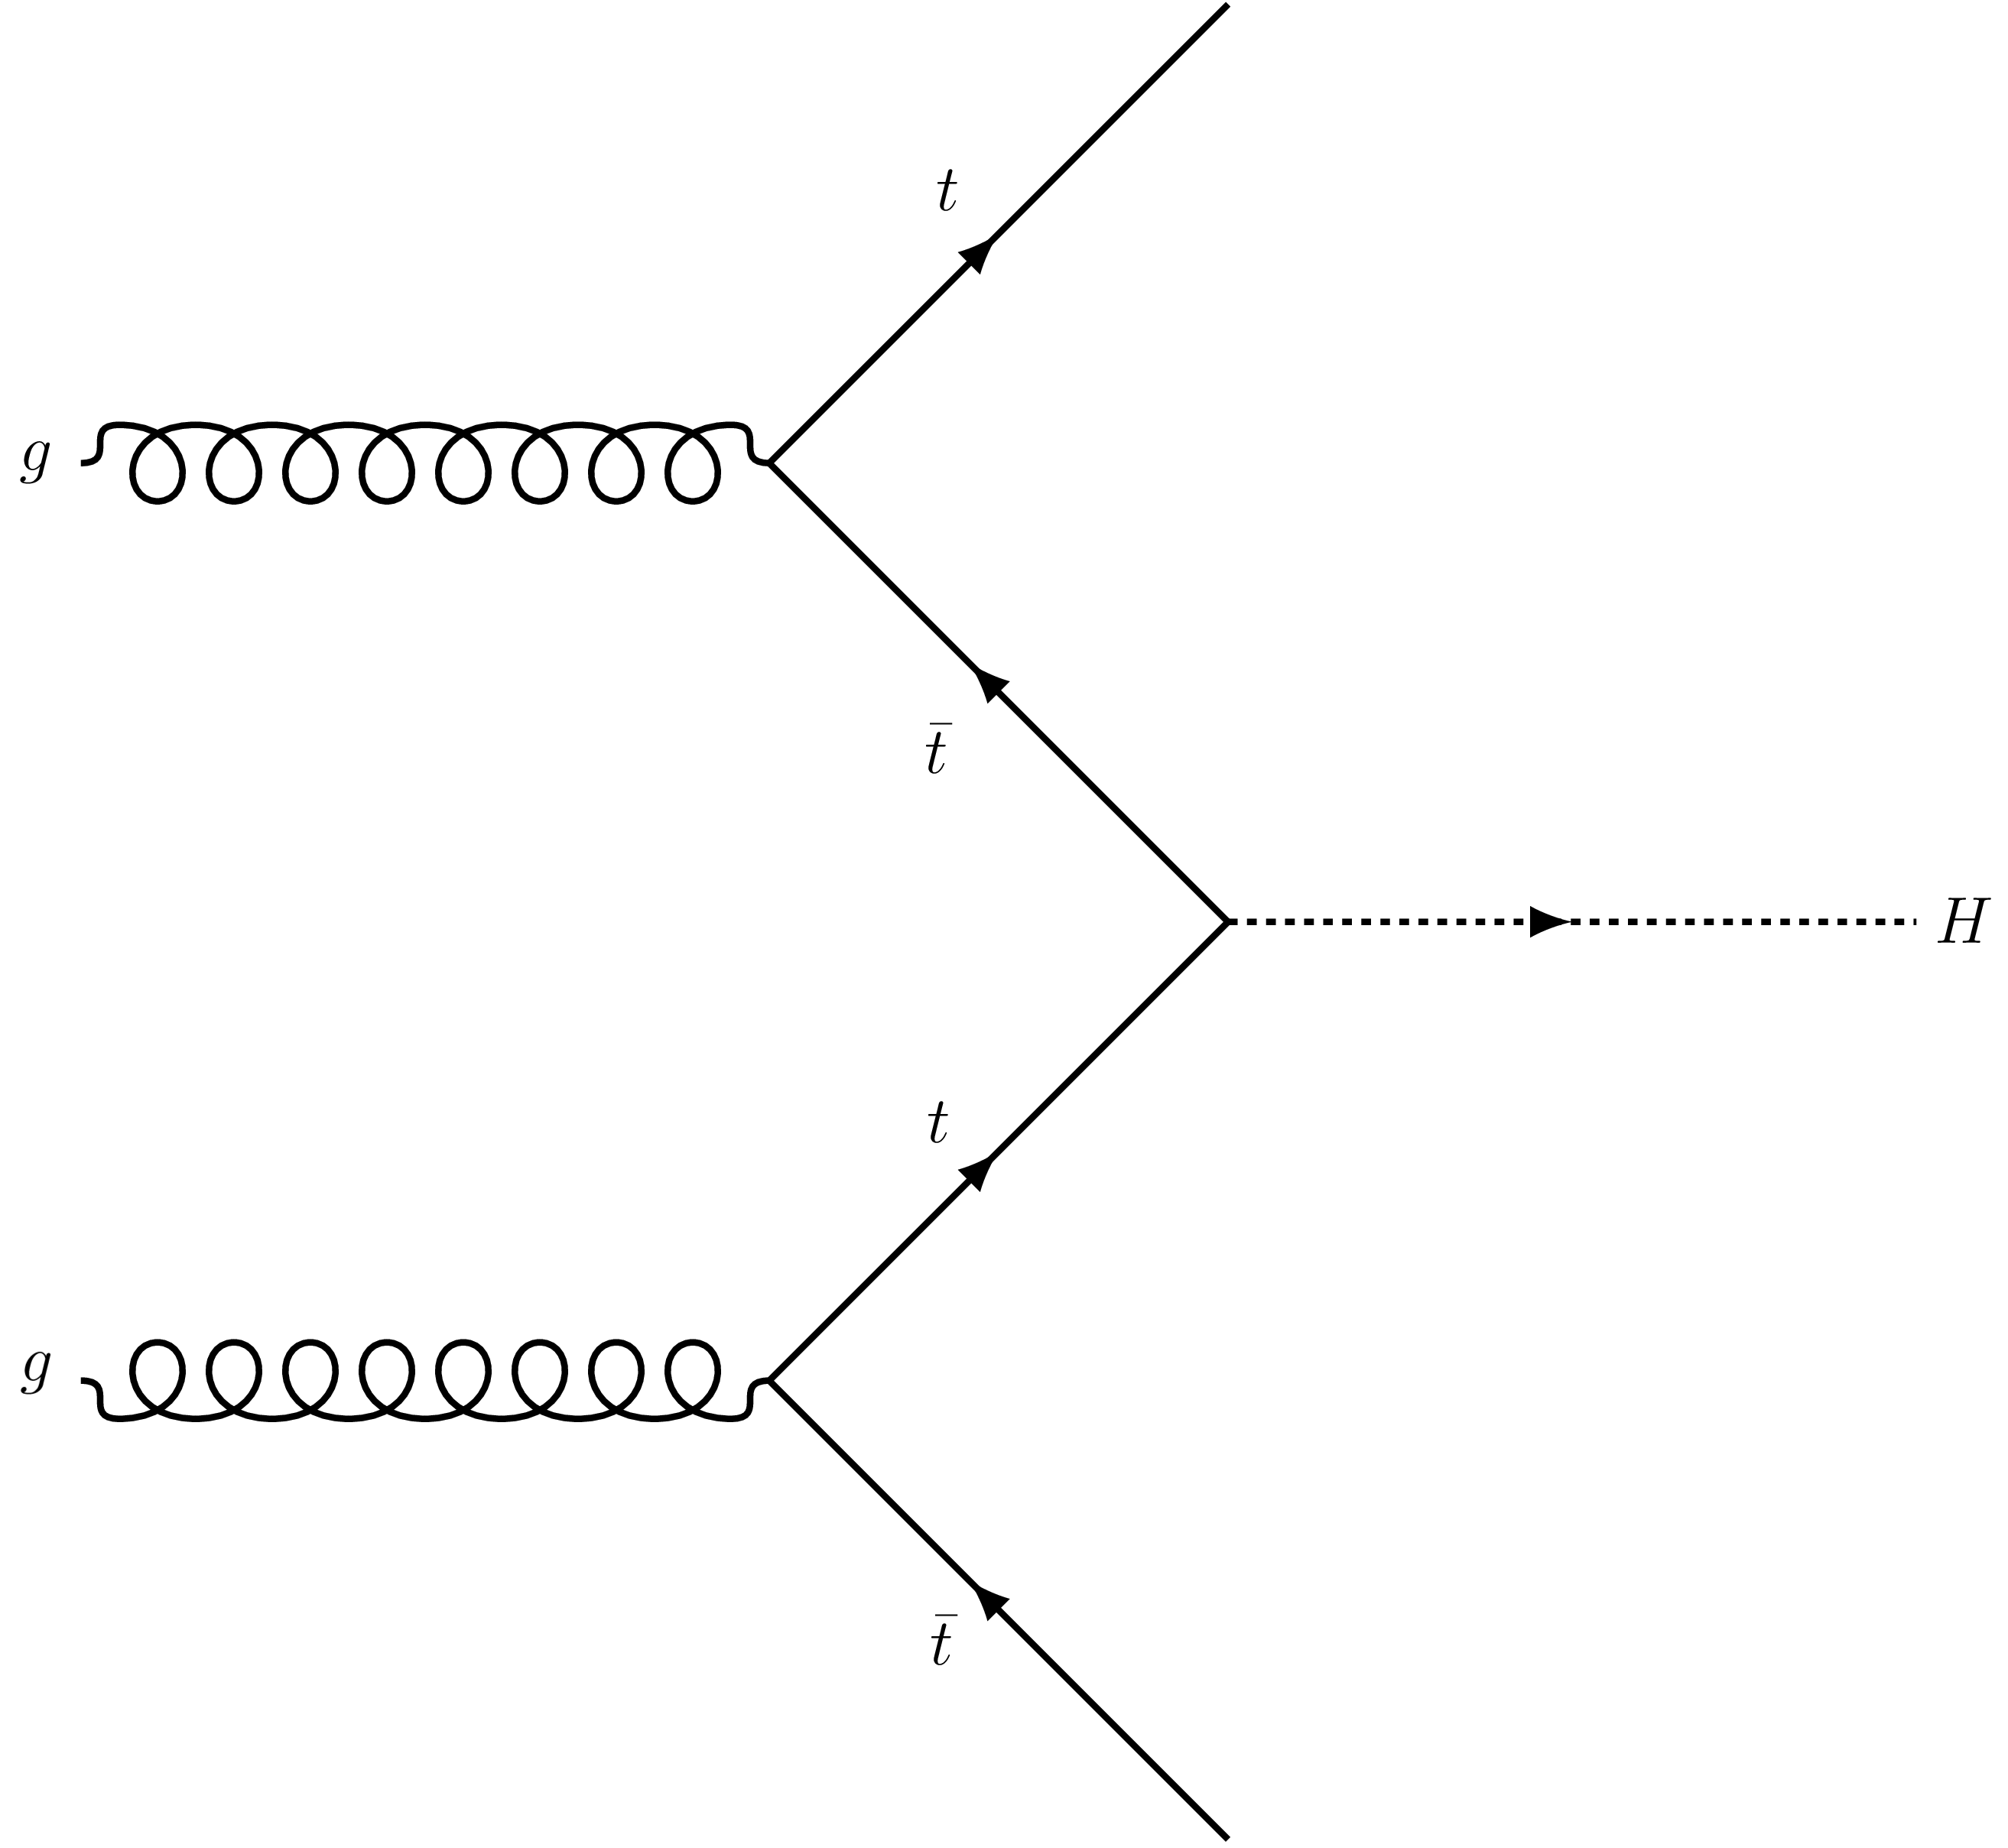
\includegraphics[width=\textwidth]{figures/feynman_diagrams/ttH.png}
        \caption{\ttH}
    \end{subfigure}
    \hfill
    \begin{subfigure}[b]{0.45\textwidth}
        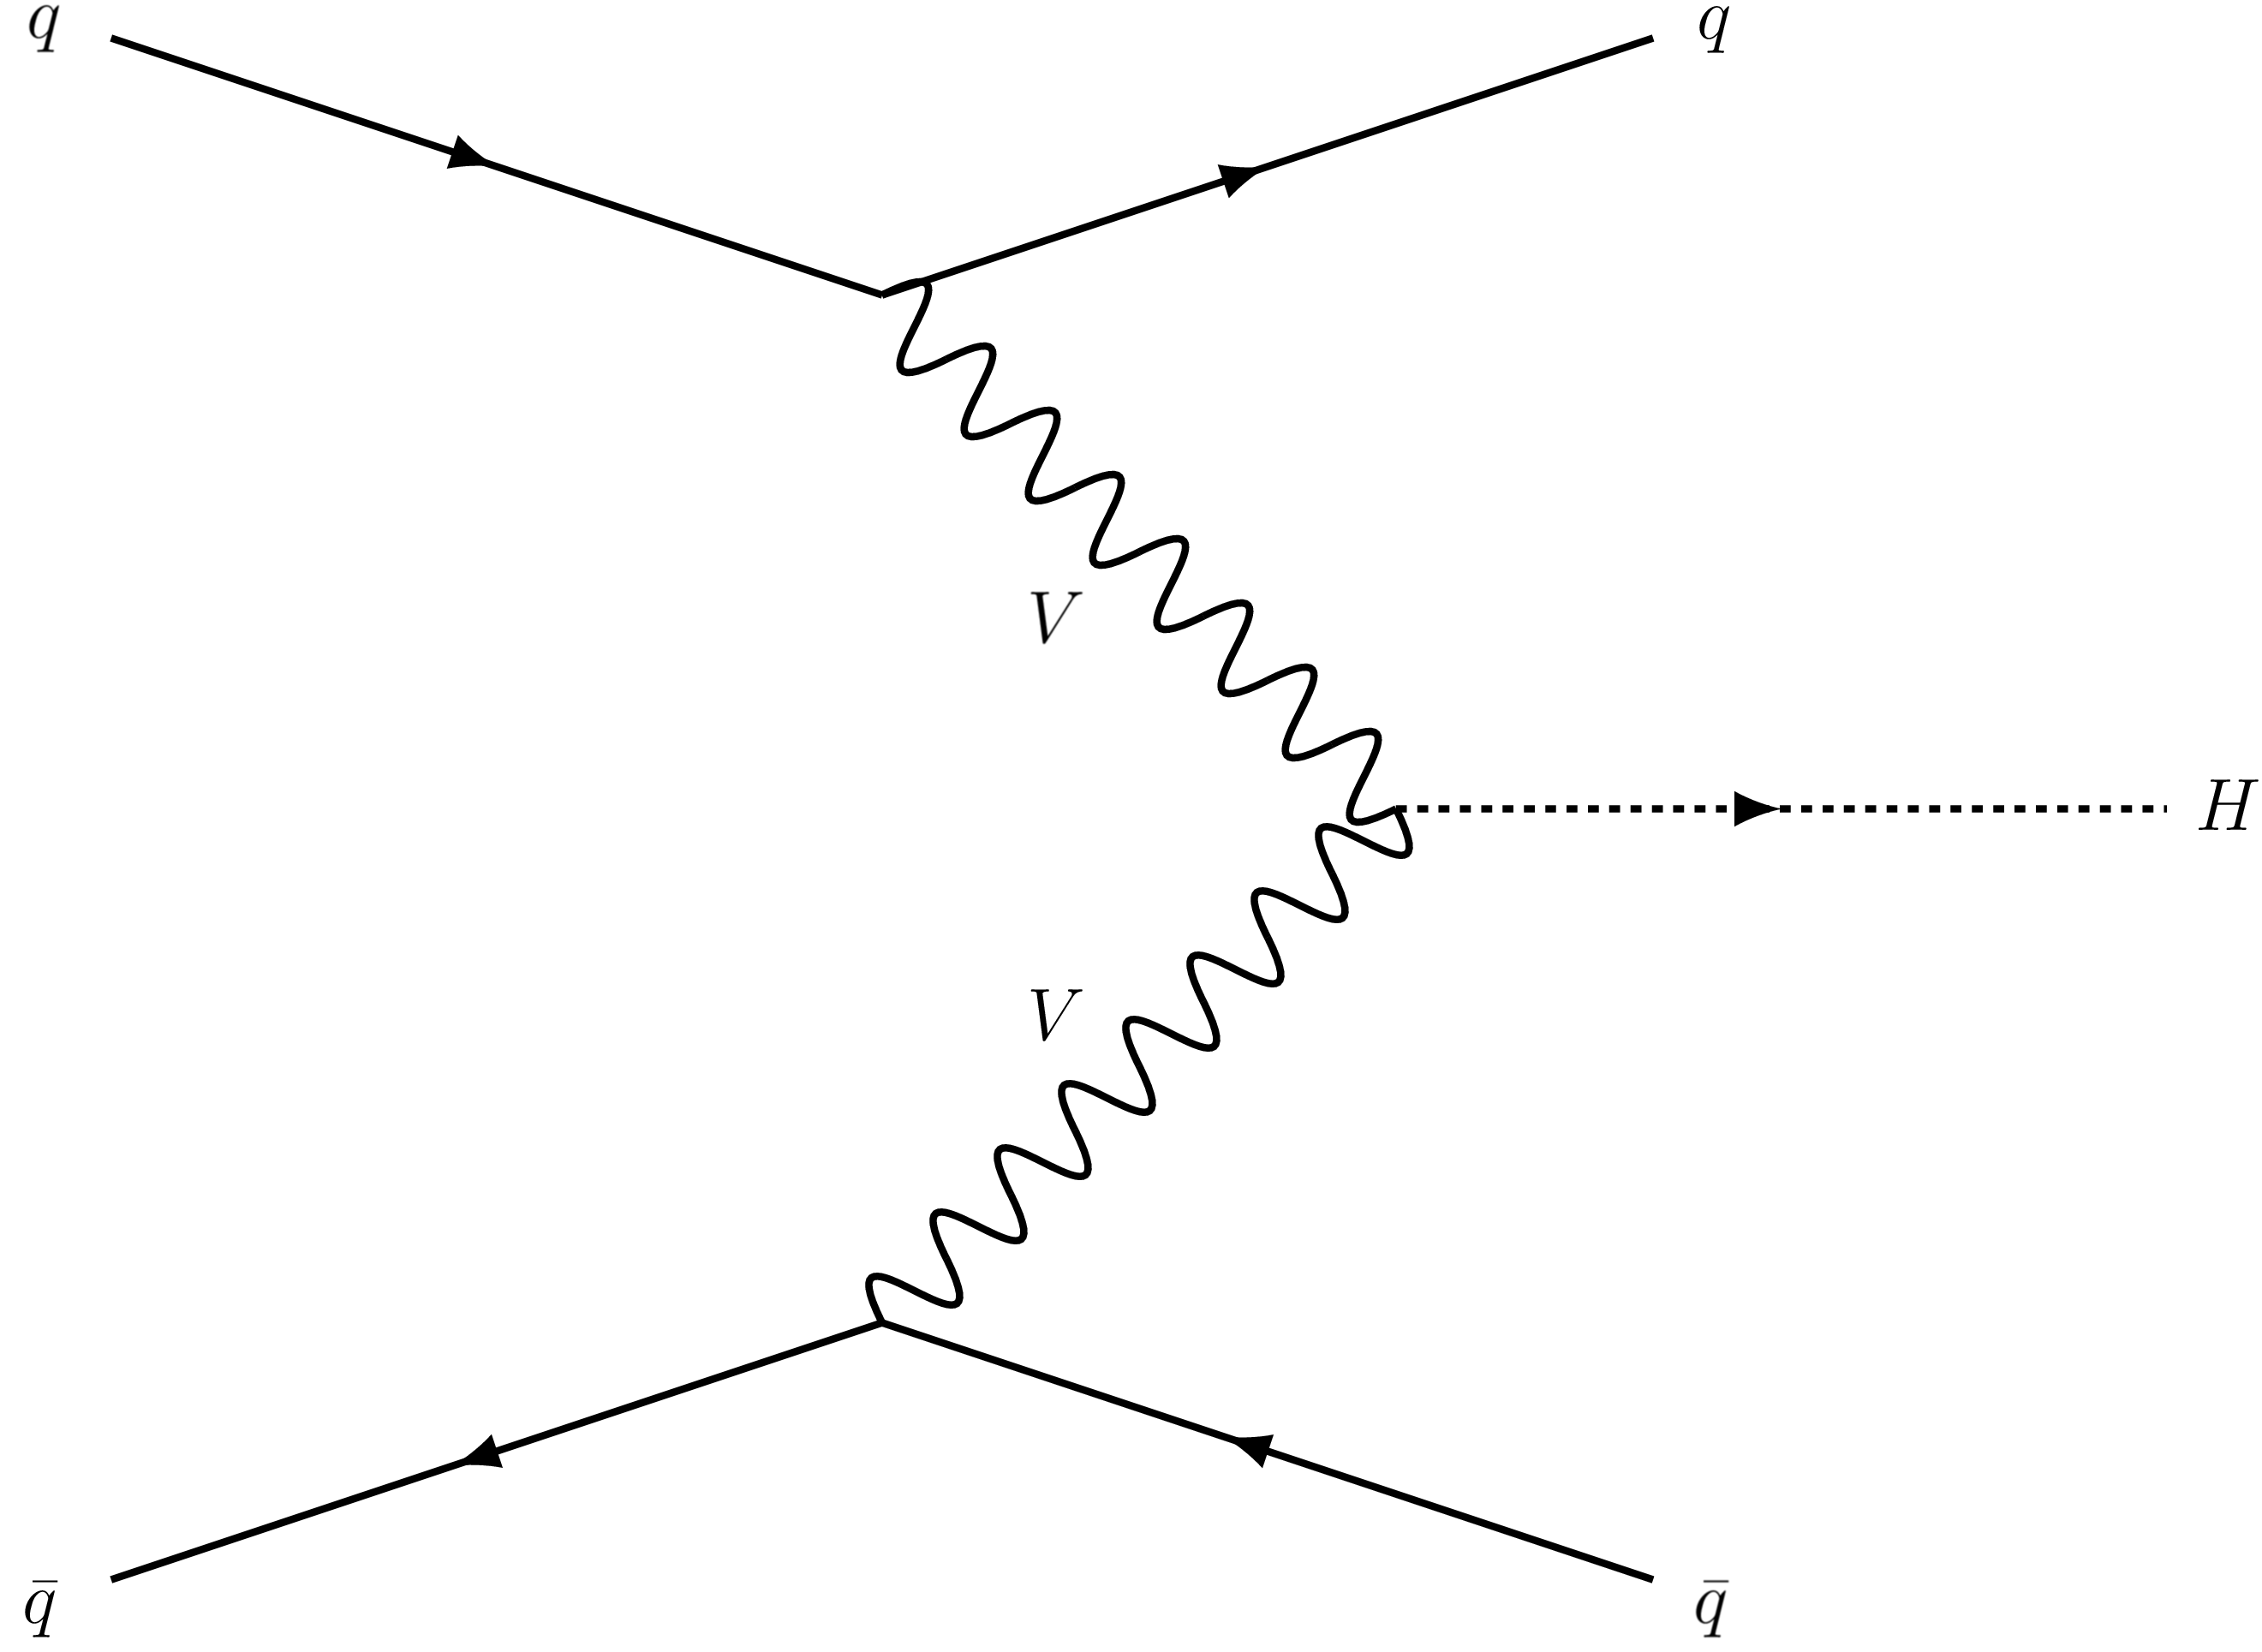
\includegraphics[width=\textwidth]{figures/feynman_diagrams/VBF.png}
        \caption{\acrshort{vbf}}
    \end{subfigure}
% blank line to start new row
    \begin{subfigure}[b]{0.45\textwidth}
        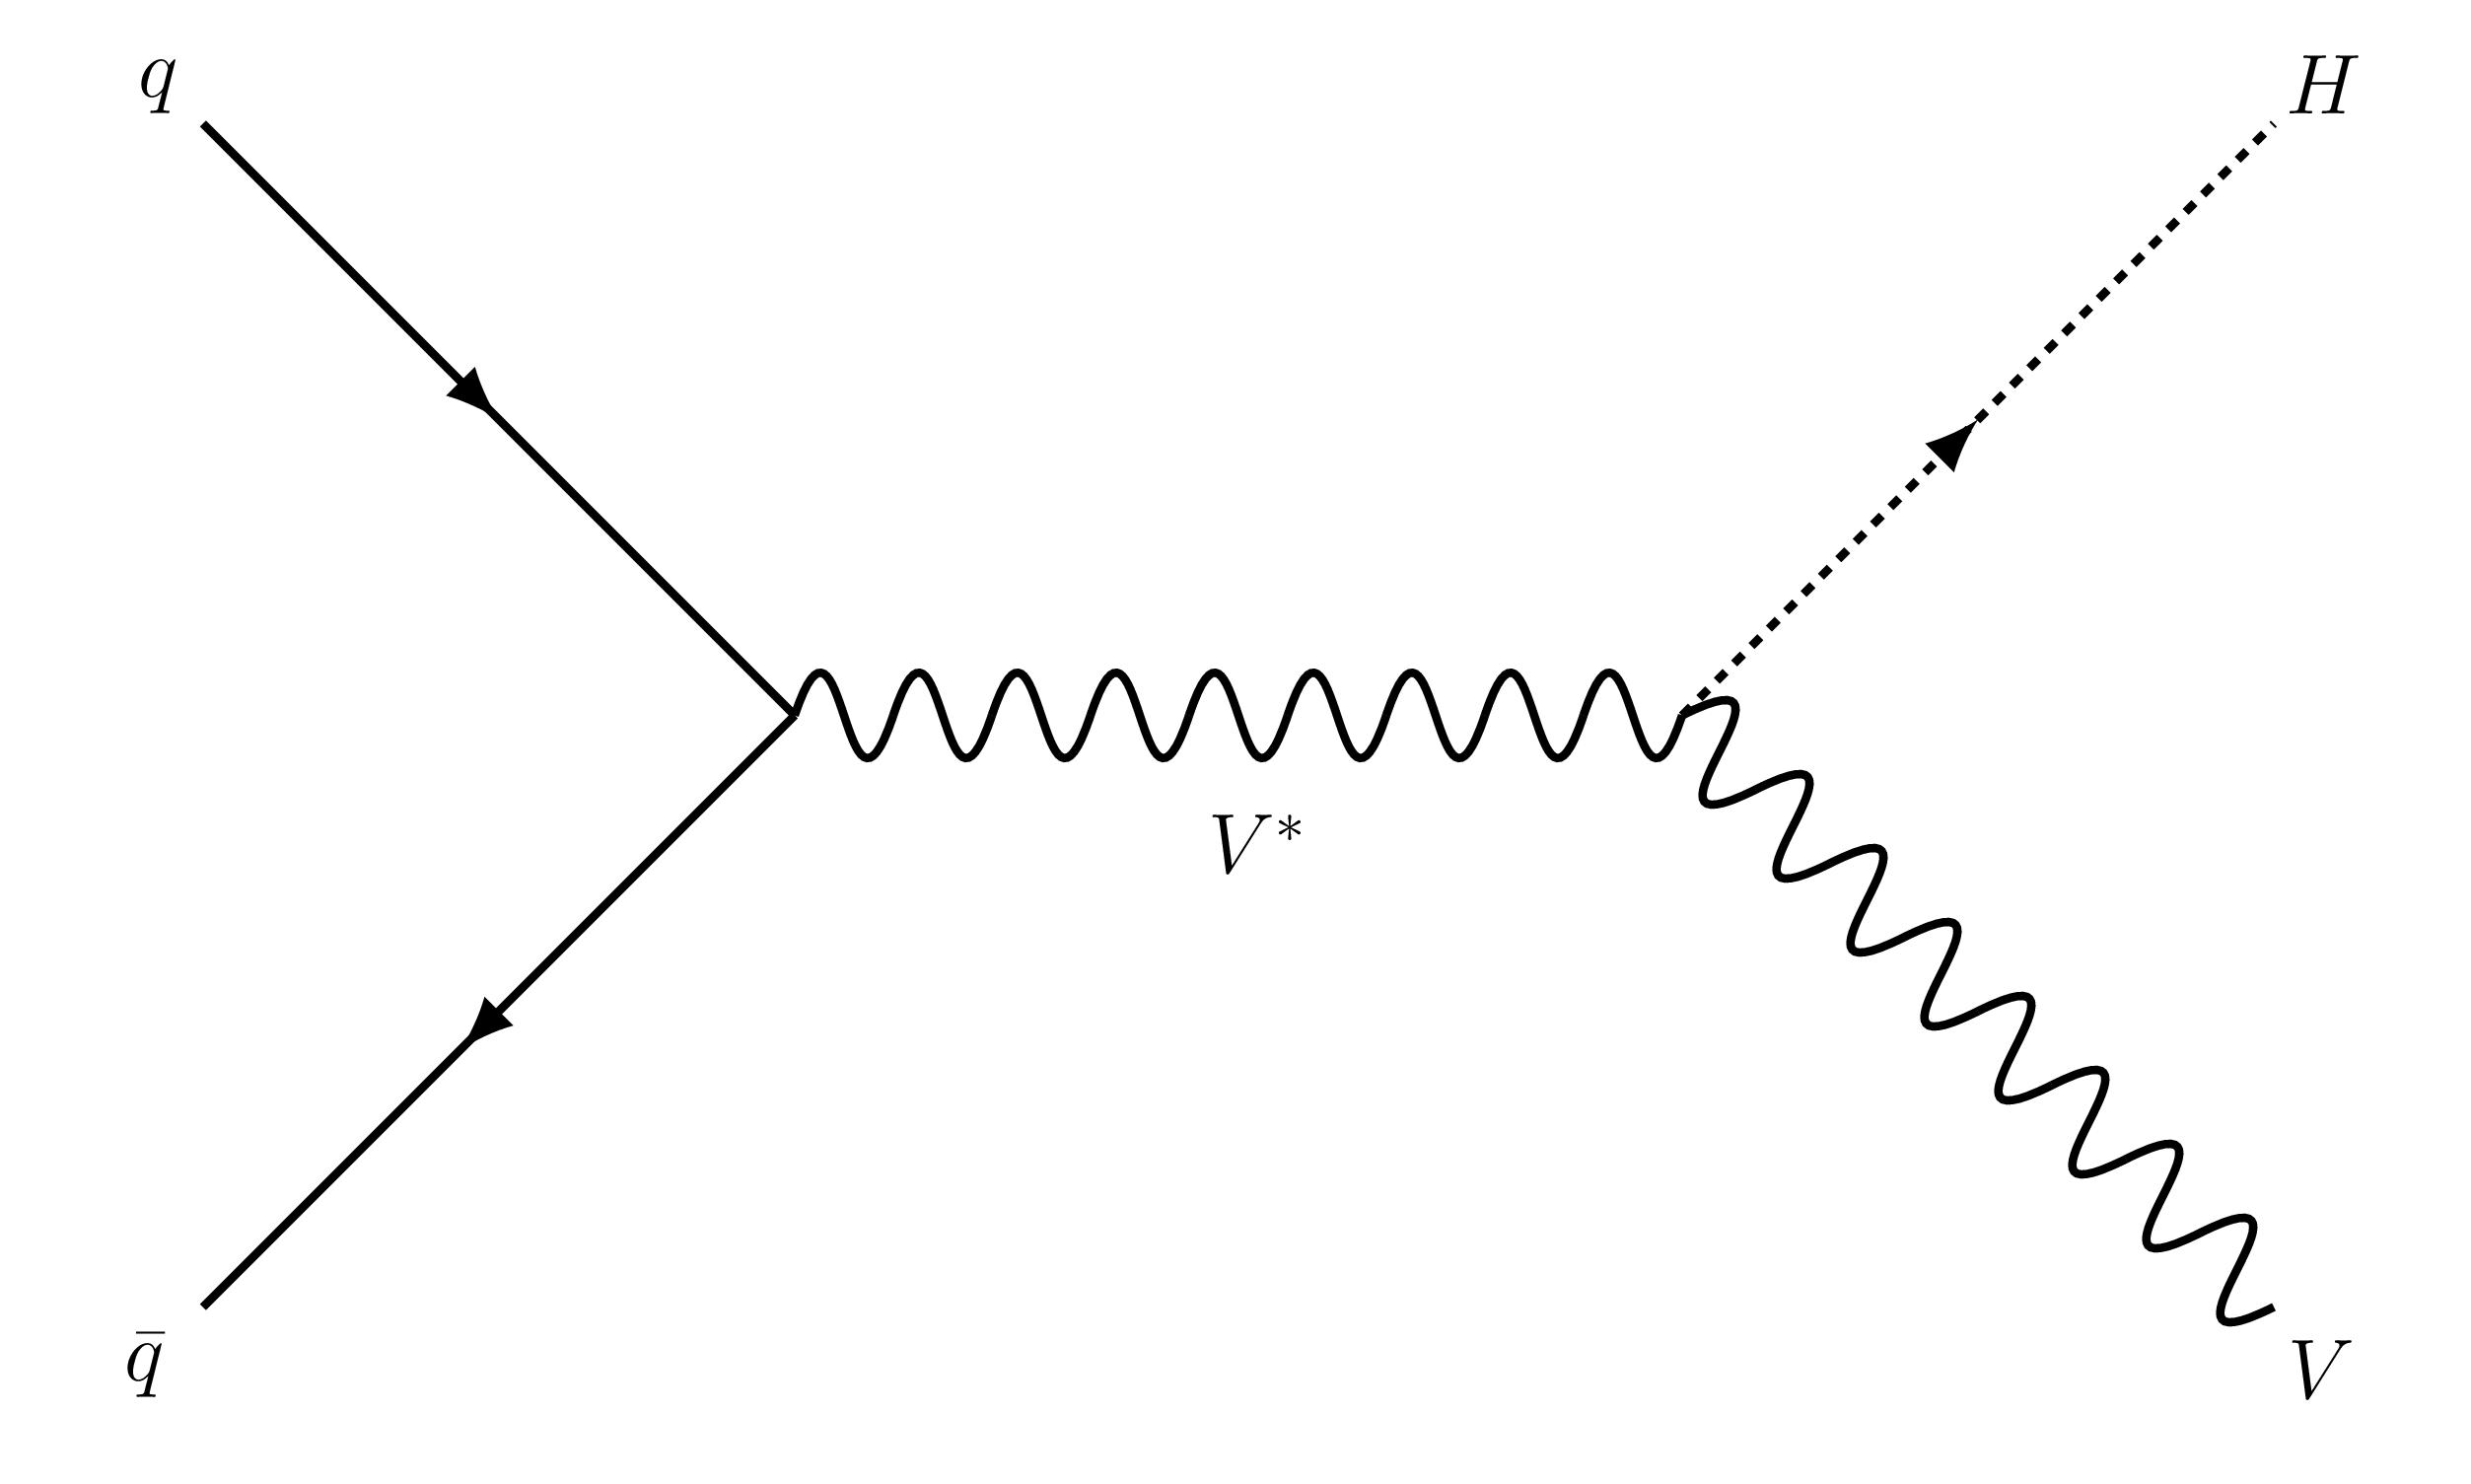
\includegraphics[width=\textwidth]{figures/feynman_diagrams/VH.png}
        \caption{\VH}
    \end{subfigure}
    \hfill
    \begin{subfigure}[b]{0.45\textwidth}
        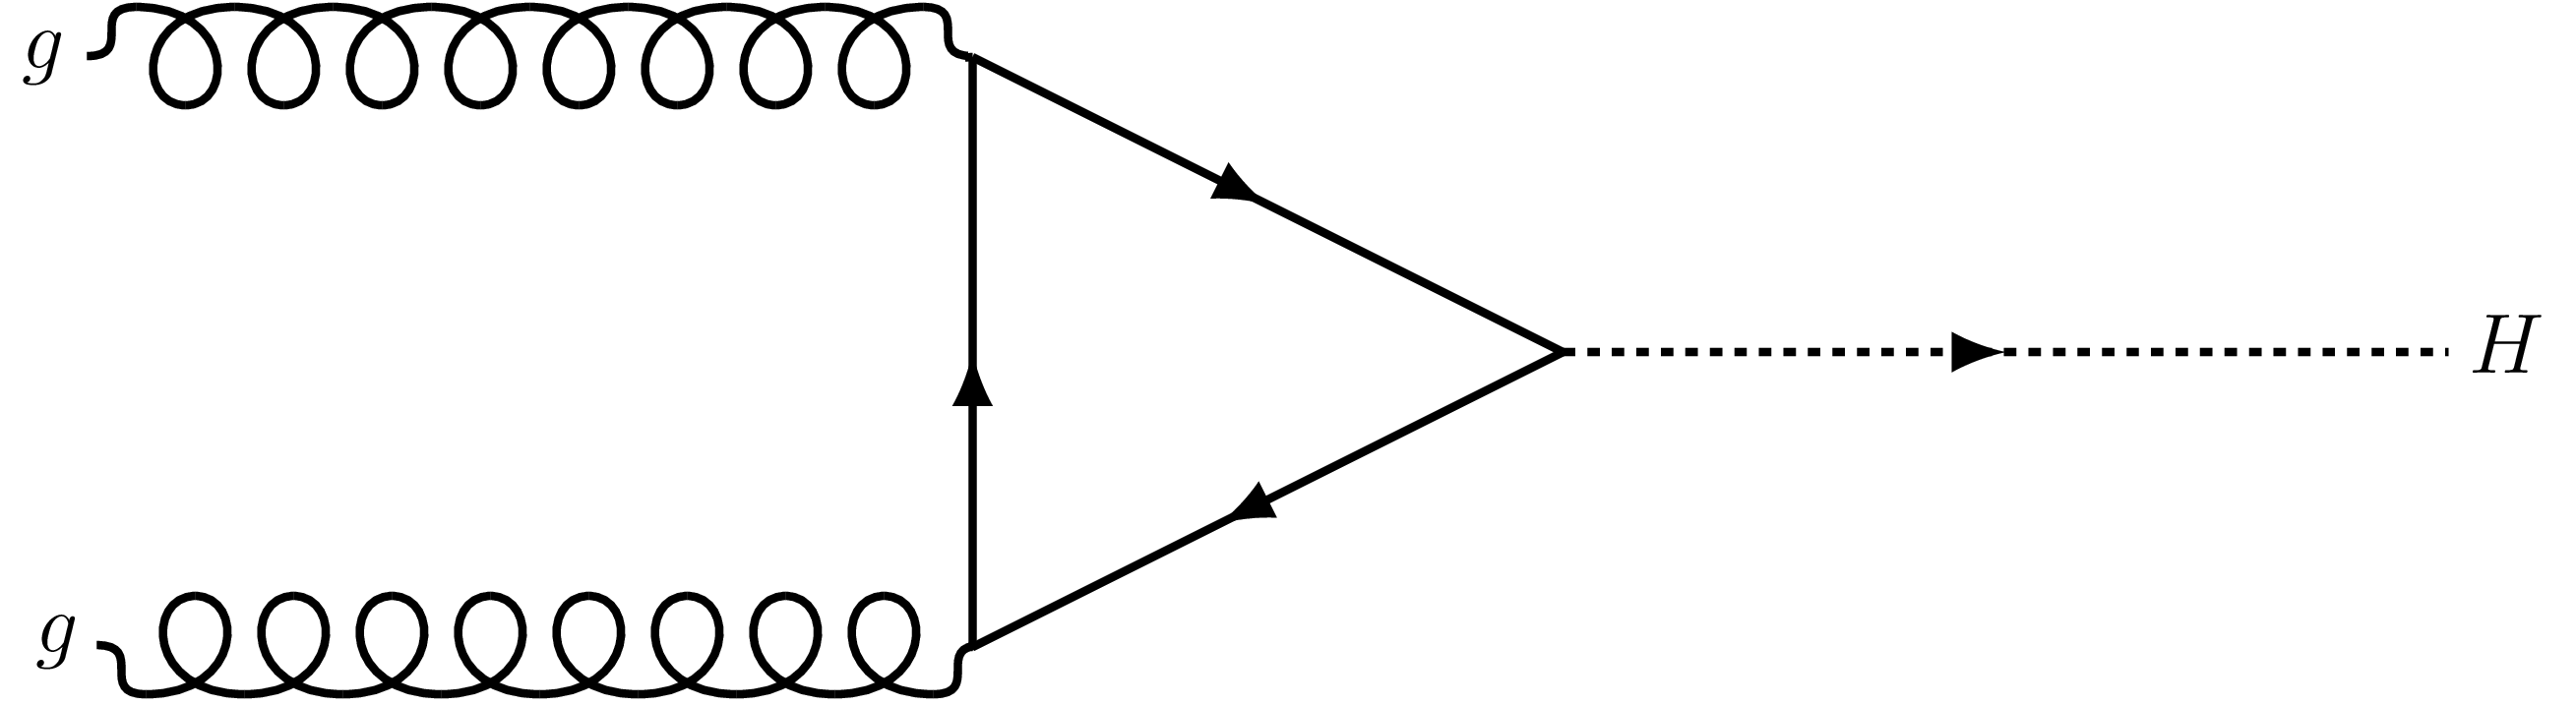
\includegraphics[width=\textwidth]{figures/feynman_diagrams/ggF.png}
        \caption{\ggF}
    \end{subfigure}
\caption[A subset of the Feynman diagrams for the four predominant production mechanisms of the Higgs boson at the LHC]{A subset of the Feynman diagrams for the four predominant production mechanisms of the Higgs boson at the \acrshort{lhc}.}
\label{fig:higgs_feynman_diagrams}
\end{figure}

% Additional diagrams for ggF are a square top loop (gluons join the two vertices on the left), where the Higgs exits at one of the vertices on the right and a gluon exits at the other. For ZH, can also have gg->ZH as well as pp->ZH. Not sure if it's worth showing them or just describing them.


%=========================================================


\subsection{Vector boson fusion (VBF)}
\label{subsec:htoinv_VBF}

A \acrshort{vbf} topology is exhibited by a \tchannel exchange of two vector bosons radiated by the incident quarks, which then to form a new particle such as a Higgs boson. Since the masses of the \PW and \PZ bosons are more than half the Higgs mass, it can easily be produced on shell. The recoil of the quarks characterises the visible system: two jets with a large combined invariant mass, usually with a large separation in pseudorapidity but small in azimuthal angle. The jets [move] in opposite directions---one in $+\eta$, the other in $-\eta$---but are usually contained in the same horizontal half of the detector.


%=========================================================


\subsection{Associated production from top quarks (\texorpdfstring{\ttH}{ttH})}
\label{subsec:htoinv_ttH}

In \ttH, two \ttbar pairs are produced. A top quark \Pqt from one pair and antiquark \APtop from the other annihilate to produce the Higgs boson. As it decays invisibly, it is the remaining \Pqt and \APtop in the event that lead to three classes of final state. The \Pqt quark decays almost exclusively to $\Pqb\PWplus$ (and $\HepProcess{\APtop \to \APqb\PWminus}$)~\cite{PhysRevD.98.030001}. In a resolved system where top quarks possess low to moderate momentum, the multitude of available \Pqb-tagging algorithms can distinguish the decays of the \Pqb quark. The products of the \PW boson is the determining factor of the final state. Hadronically-decaying $\PW\text{s}$ ($\HepProcess{\PW \to \Pquark\APquark}$), of course, produce pairs of jets. But they can also decay into a lepton and neutrino. The final states then all have \ptmiss and up to two \glspl{bjet} in common. Several \glspl{jet} may accompany them (the hadronic channel), or fewer \glspl{jet} with a single lepton (the \emph{semi-leptonic} channel), or two leptons (the dileptonic channel). The magnitude and direction of the \ptmiss in the latter two channels may be affected by the neutrinos, depending on their direction and energy.

In a boosted system where the top quarks have significant \pt, it is often difficult to tag \glspl{bjet}, especially if one is searching in the hadronic channel. Recently-developed algorithms can assist in this case by inspecting AK8 \glspl{jet}---objects clustered with the \gls{antikt} using a radius parameter of 0.8 instead of the usual 0.4. The \deepakeight algorithm, discussed in further detail in Chpt.~\ref{subsec:htoinv_deepak8}, is used in the analysis to classify boosted topologies originating from \Pqt quarks as well as \PVec bosons to identify \ttH events.


%=========================================================


\subsection{Associated production from a vector boson (\texorpdfstring{\VH}{VH})}
\label{subsec:htoinv_VH}

A Higgs boson is radiated by the vector boson \PVec in the \VH mechanism. Parallels can be drawn with \ttH as the decay of the \PVec determines the search channel. Resolved and boosted systems are also possible. In the resolved case, a dijet pair with an invariant mass close to that of the parent boson would distinguish the hadronic channel. \Pqb-taggers can be exploited if the decay is to a \Pqb quark, i.e., $\HepProcess{\PWplus \to \APqb\Pquark_{\Pup}}$,\footnote{I'm not sure what the symbol is (if there even is one) for an up-type quark. Maybe $\Pquark_{\Pup, \Pcharm}$ to be more specific, or $\Pquark_{\uparrow}$?} $\HepProcess{\PWminus \to \Pqb\APquark_{\Pup}}$, or $\HepProcess{\PZ \to \Pqb\APqb}$. Single lepton channels are possible for \WH and dilepton for \ZH. For a boosted \PVec, one expects the products to the collimated into a single AK8 \gls{jet}, at least in the hadronic channel. As with \ttH, we take advantage of the \deepakeight tagger to capture these scenarios. 


%=========================================================


\subsection{Gluon-gluon fusion (\texorpdfstring{\ggF}{ggF})}
\label{subsec:htoinv_ggF}

Despite \ggF having the largest cross section of the four modes, its upper limit on $\BRof{\higgstoinv}$ is the weakest. This process [produces] a Higgs boson through their fusion, normally mediated by a top quark since it has the largest coupling to the Higgs. With no additional final state particles, searches for this production mode usually involve initial state radiation from the gluons or the loop. As such, the signature is at least one \gls{jet} and \ptmiss.


%=========================================================


\section{Results of previous searches}
\label{sec:htoinv_prev_results}

Many previous analyses have investigated the \higgstoinv decay, in some cases from dedicated searches, but often as an afterthought or interpretation of the main analysis. \acrshort{vbf} is the most sensitive production mode. This is demonstrated in Tab.~\ref{tab:hinv_br_limits} by the upper limits [achieved] compared to the other mechanisms. In Ref.~\citenum{Sirunyan:2018owy}, a combination was performed over all the productions modes detailed in the table (with the exception of \ttH). Using the recent 2016 measurements as well as data taken from Run-1 and 2015, this combined observed upper limit [sits at] 19\,\%, while the expected is 15\,\%. With only data from Run-1 and 2015---the previous combination---yields the observed and expected upper limits of 24\,\% and 23\,\%, respectively~\cite{Khachatryan:2016whc}.

\begin{table}[htbp]
    \centering
    \begin{tabular}{lllcc}
        \hline
        Targeted mode & Analysis & Final state & Observed UL & Expected UL\\\hline
        \acrshort{vbf} & Ref.~\citenum{Sirunyan:2018owy} & $\text{\acrshort{vbf}-\glspl{jet}} + \ptmiss$ & 33\,\% & 25\,\% \\
        $\ZH(\HepProcess{\PZ \to \Plepton\Plepton})$ & Ref.~\citenum{Sirunyan:2017qfc} & $\PZ(\HepProcess{\to \Plepton\Plepton}) + \ptmiss$ & 40\,\% & 42\,\% \\
        $\ttH$ & Ref.~\citenum{CMS-PAS-HIG-18-008} & $\ttbar(\HepProcess{\to \text{\glspl{jet}}/\Plepton/\Plepton\Plepton}) + \ptmiss$ & 46\,\% & 48\,\% \\
        $\VH(\HepProcess{\PVec \to \Pquark\APquark})$ & Ref.~\citenum{Sirunyan:2017jix} & $\PVec(\HepProcess{\to \Pquark\Pquark}) + \ptmiss$ & 50\,\% & 48\,\% \\
        $\ggF$ & Ref.~\citenum{Sirunyan:2017jix} & $\text{\glspl{jet}} + \ptmiss$ & 66\,\% & 59\,\% \\\hline
    \end{tabular}
    \caption[The most recent searches for invisibly decaying Higgs bosons with 2016 data from CMS, and the upper limits on the \higgstoinv branching ratio at 95\,\% confidence level achieved]{The most recent searches for invisibly decaying Higgs bosons with 2016 data from \acrshort{cms}, and the upper limits (UL) on the \higgstoinv branching ratio at 95\,\% confidence level achieved. Only the \acrshort{vbf} analysis is a dedicated search, while the others are interpretations of the results obtained in their respective primary analyses. For the $\ttH$ analysis, the hadronic (\glspl{jet}), semi-leptonic (\Plepton), and dileptonic ($\Plepton\Plepton$) channels were combined.}
    \label{tab:hinv_br_limits}
\end{table}


%=========================================================


\section{Overview of the analysis}
\label{sec:htoinv_analysis_overview}

The analysis discussed in the remainder of the chapter is a dedicated search for invisibly decaying Higgs bosons in hadronic final states, incorporating all four of the production modes [discussed] above from the outset. In contrast to many of the previous analyses that separately set limits on $\BRof{\higgstoinv}$ by reinterpretation, our approach has many benefits. A simultaneous search for all of the production modes allows us to construct search regions to target each one, building in orthogonality to avoid overlap between them. Data and simulation samples, recipes for systematic uncertainties, the analysis framework, and results can all be shared to provide a cohesive and consistent environment from which to perform the analysis. As well as streamlining the process of the final combination over each production mechanism, communication when [setting up] the analysis ensures each can cover as much phase space as possible without the trouble of overlap or contamination.

Direct collaboration amongst several institutes divides up the task appropriately. Researchers at the University of Bristol, such as myself, and LLR (\emph{Laboratoire Leprince-Ringuet, \'{E}cole Polytechnique, Universit\'{e} Paris-Saclay}) focus on \ttH and the resolved \VH modes. Those at Imperial College London, who have a long history with the \acrshort{vbf} search~\cite{Chatrchyan:2014tja,Sirunyan:2018owy}, assume responsibility of this mechanism. Researchers at Boston University---who have previously been involved in \acrshort{bsm} analyses with interpretations in invisibly decaying Higgs bosons~\cite{Khachatryan:2016mdm,Sirunyan:2017jix}---specialise in monojet and mono-\PVec searches. This makes them naturally suited to investigating the boosted aspect of \VH, and \ggF.

Emphasis will be placed on the non-VBF modes, particularly \ttH and resolved \VH, as I have had direct involvement in those aspects of the analysis. Before Boston University joined the analysis, we also studied the boosted \VH and \ggF mechanisms. Accordingly, they will also be given some attention. The object definitions are discussed in Chpt.~\ref{sec:htoinv_objects}, followed by the event selection in Chpt.~\ref{sec:htoinv_event_selection}. Definitions of the regions and categories are illustrated in Chpts.~\ref{sec:region_definitions} and \ref{sec:htoinv_categorisation}, respectively. The data from \acrshort{cms} and from simulation, along with required corrections and systematic uncertainties are acknowledged in Chpt.~\ref{sec:htoinv_data_sim}. Methods for estimating the background processes in the signal region are described in Chpt.~\ref{sec:htoinv_background_est}. The incorporation of these and the aforementioned sections in the statistical treatment of are presented in Chpt.~\ref{sec:htoinv_satistical_treatment}, before the results of the analysis in Chpt.~\ref{sec:htoinv_results}.

% Given the \acrshort{lhc} is a \emph{hadron} collider, processes with hadronic channels are the natural choices.\footnote{Or should I say ``most sensitive''?} \Gls{met} from the purely-invisible decay of the Higgs---and hadronic activity from the particles associated with the production mechanism---constitute the [final state], often known as a ``\text{\glspl{jet}} + \ptmiss$'' search.


%=========================================================


\section{Object definitions}
\label{sec:htoinv_objects}


%=========================================================


\section{Event selection}
\label{sec:htoinv_event_selection}

The event selection aims to strike the balance between rejecting as many background events while maintaining as great a signal sensitivity as possible. The preselection, in Chpt.~\ref{subsec:htoinv_preselection}, is applied to data and simulation in all regions and categories to do just that. Filters to reject potentially-mismeasured events and those that lead to incorrect \ptmiss calculations are documented in Chpt.~\ref{subsec:htoinv_other_filters}. The region- and dataset-specific triggers are described in Chpt.~\ref{subsec:htoinv_trigger_sel}.


%=========================================================


\subsection{Preselection}
\label{subsec:htoinv_preselection}


%=========================================================


\subsection{Additional filters}
\label{subsec:htoinv_other_filters}


%=========================================================


\subsubsection{\texorpdfstring{\ptmiss}{MET} filters}
\label{subsubsec:htoinv_met_filters}


%=========================================================


\subsection{Trigger selection}
\label{subsec:htoinv_trigger_sel}


%=========================================================


\section{Signal region, control region, and sideband definitions}
\label{sec:region_definitions}


%=========================================================


\subsection{The signal region}
\label{subsec:htoinv_signal_region}


%=========================================================


\subsection{Control regions}
\label{subsec:htoinv_control_regions}

% Mention that the leptons/photons are removed from the MET calculation.


%=========================================================


\subsection{Sidebands to the signal region}
\label{subsec:htoinv_sidebands}


%=========================================================


\section{Categorisation of the non-VBF production modes}
\label{sec:htoinv_categorisation}


%=========================================================


\subsection{Classifying boosted topologies from top quarks, \texorpdfstring{\PW}{W} and \texorpdfstring{\PZ}{Z} bosons}
\label{subsec:htoinv_deepak8}


%=========================================================


\section{Data and simulation}
\label{sec:htoinv_data_sim}


%=========================================================


\subsection{Data}
\label{subsec:htoinv_data}

The data collected by the \acrshort{cms} experiment that is used in the analysis corresponds to an integrated luminosity of 137.19\fbinv, and recorded from 2016--2018. A breakdown by year is given in Tab.~\ref{tab:lumis_lhc_cms}. Data is split into ``primary datasets'' that are grouped by the class of \acrshort{hlt} path that an event triggered. The signal region, \acrshort{qcd} sidebands, and muon \glspl{CR} use the primary dataset composed of \etmiss and \htmiss combination triggers, where muons are excluded from the sums. The datasets [used] in the electron and photon \glspl{CR} consist of triggers based on electron and photon object thresholds. These were separate for 2016 and 2017, then merged for 2018.

Some serious issues arose during Run-2 that had to be mitigated after the events were reconstructed. With the high collision rate at \acrshott{cms}, in order to properly correlate the hits in the subdetectors with the correct particles and events they are attributed to, the timing infrastructure must be very precise. Timing scans are conducted frequently during runs to correct or compensate for any shifts that may occur. However, in 2016 and 2017, the gradual timing drift in the \acrshort{ecal} was not correctly propagated to the \acrlong{l1} trigger primitives. This resulted in a significant fraction of them in the forward direction (as the effect increases with $\eta$) being mistakenly associated to the previous bunch crossing: \emph{pre-firing}. One rule at \acrshort{l1} forbids two consecutive bunch crossings from firing signals to the trigger system. But, a consequence of this---in addition to not finding the primitive in the nominal bunch crossing---is that events can be vetoed if a significant amount of \acrshort{ecal} energy is found in the $\text{2} < \abseta < \text{3}$ part of the end cap. It is observed only in data, and so a correction is applied to \acrshort{mc} (see Chpt.~[REF]) to account for the effect.
% Pre-firing: https://twiki.cern.ch/twiki/bin/viewauth/CMS/L1ECALPrefiringWeightRecipe, https://indico.cern.ch/event/764279/

In 2018, a sector of the \acrshort{hcal} end cap lost power and left the approximate area $\eta = [-3.0, -1.4]$, $\phi = [-1.57, -0.87]$ uncovered for the remainder of the year. Of the 59.7\fbinv recorded and certified for use in 2018, 38.6\fbinv were affected. With this section missing, it is more difficult to accurately record the properties of \glspl{jet}, and therefore reliably calculate \ptmiss. Studies performed showed an excess in data in the affected area of the $\phi(\ptmiss)$ distribution of many of our regions and categories. To mitigate this issue, the following cuts were added to the preselection: XXX.


%=========================================================


\subsection{Simulated signal processes}
\label{subsec:htoinv_signal}

All \acrlong{mc} datasets used in this analysis was produced centrally by experts in \acrshort{cms} as described in Chpt.~\ref{subsec:cms_mc}. The signal samples are generated at \acrshort{nlo} with the \POWHEG generator interfaced with \PYTHIAEIGHT. When reweighting events for their cross section, they are specified at \acrshort{nnlo}.\footnote{Should I give a table or something of the cross sections for the signal samples?} The samples are produced with a Higgs boson mass of $m_{\PH} = \text{125}\GeV$. The vector bosons in each of the \VH channels decay to $\Pquark\APquark$. When simulating 2016 data, the tuning of the shower parameters in \PYTHIA was labelled \textsc{cuetp8m1} (the latest available), whilst for 2017 and 2018 datasets the newer \textsc{cp5} version was used.


%=========================================================


\subsection{Simulated background processes}
\label{subsec:htoinv_background}

\acrlong{mc} datasets for many processes are used in the analysis to accurately represent the \acrlong{sm} background. Every one uses \PYTHIAEIGHT to hadronise the events generated by the hard scatter. The underlying event tune applied in the hadroniser follows the same prescription as with signal---\textsc{cuetp8m1} is used for 2016 while \textsc{cp5} is used thereafter. The only exception is the $\ttbarpjets$ background, for which \emph{all} samples were generated with the \textsc{cp5} tune. They are described as follows:

% What words can I use instead of "process" as I seem to use it a lot here? Decay/dataset/mechanism/background?

\begin{easylist}[itemize]
    \easylistprops
    & Drell-Yan $(\HepProcess{\PZ \to \Plepton\Plepton}) \plusjets$: The Drell-Yan process occurs when the quark of one incident proton annihilates with the antiquark in the oncoming proton, producing a neutral vector boson (a \PZ in this case) from a \acrshort{qcd} vertex. The \PZ boson decays to a lepton pair, so while absent in the signal region, is the dominant background in the dilepton control regions used to model the \ztonunupjets process. The datasets are generated at \acrshort{lo} accuracy with \MGvATNLO, where a dilepton mass cut of 50\GeV is applied.

    & Multiboson: This process encompasses the production two (diboson) or three (triboson) electroweak bosons from \acrshort{qcd}(?) vertices. They may decay leptonically, also producing neutrinos in the case of \PW bosons, but also hadronically, producing \glspl{jet}. A mixture of the two in an event will lead to similar signatures to that of the signal. The diboson processes are both generated and showered with \PYTHIAEIGHT at \acrshort{lo}. Triboson events, on the other hand, \MGvATNLO at \acrshort{nlo} accuracy models the hard scatter.

    & Electroweak $\PVec + \text{2 jets}$: The production of electroweak bosons from an electroweak vertex is a minor background in the signal region. But as above, they may produce genuine \ptmiss from the decay of the \PVec. The datasets are generated at \acrshort{lo} with \MGvATNLO. % Mention something about the M-50 cut (if I can find out what it is), and maybe about the Vs only decaying into lnu, ll and nunu (perhaps that's what the 'electroweak' vertex means)

    & \singlePhotonCr: Events with photons are vetoed in the signal region. However, this is the dominant background in the \singlePhotonCr \gls{CR}, that predicts the \ztonunupjets contribution to the signal region, along with the double lepton regions. This dataset is generated at \acrshort{lo} with \MGvATNLO, where the $\Delta R > \text{0.4}$ between a photon and jet is required.

    & \acrshort{qcd} multijet: The most common type of event produced in $\Pp\Pp$ collisions at the \acrshort{lhc} is several \glspl{jet} from \acrshort{qcd} vertices. These typically do not have large \ptmiss, but are prone to mismeasurements that can artificially increase it. As such, they serve as a non-negligible background in the analysis. The datasets are produced at \acrshort{lo} by \MGvATNLO.

    & Single top: Events with a single top quark are a subdominant background in the analysis, but are important to consider, especially in the \ttH categories. These electroweak-induced processes include \schannel and \tchannel production where a \emph{four-flavour scheme}~\cite{Krauss:2017wmx} in the event generator is used for treatment of \Pqb quarks. This approach considers the \Pqb as massive, and as such, may only enter the final state. Associated production with a \PW boson (known as $\Ptop\PW$) is also considered with a five-flavour scheme, i.e., \Pqb quarks may be considered massless and can appear in both the initial and final states. For all of these channels, the events are produced at \acrshort{nlo}. Modelling the hard scatter for the \schannel diagram is performed with \MGvATNLO. The \tchannel and $\Ptop\PW$ mechanisms are generated with \POWHEG, with the former decaying the $\PW$ exchanged by the initial state $\Pqb$ and $\Pquark$ with \MADSPIN~\cite{Artoisenet:2012st} to include spin correlations.

    & \ttbarpjets: The \acrshort{qcd}-induced process presents a major background, especially in the \ttH categories. Large \ptmiss can arise in scenarios where the leptons in a decay are ``lost'' from misidentification or is outside the bounds of the detector acceptance. The three channels (hadronic, semi-leptonic, and dileptonic) are modelled with \POWHEG at \acrshort{nlo} accuracy.

    & $\ttbar X \plusjets$: These are rare processes where a boson $X$ ($\Pphoton$, $\PW$, $\PZ$, $\PH$) is produced in association with a \ttbar pair. Several combinations of the decays of the \ttbar and $X$ are covered. All of the datasets are generated at \acrshort{nlo}. The $\ttbar \PVec \plusjets$ and $\ttbar \PW \plusjets$ datasets use \MGvATNLO with the ``FxFx'' jet matching scheme for the hard scatter, and decay the particles with \MADSPIN. $\ttbar \PZ \plusjets$ uses \MGvATNLO without the two aforementioned additions. Meanwhile, $\ttH \plusjets$ (where the \PH decays to visible states) is generated with \POWHEG.

    & \wtolnupjets: A \acrshort{qcd}-induced process, this background is dominant in the single lepton \glspl{CR}. If the lepton is lost, the \ptmiss can be be inflated and lead to a significant contribution in the signal region. The datasets are produced at \acrshort{lo} with \MGvATNLO.

    & \ztonunupjets: From the presence of neutrinos, the genuine \ptmiss from this process is a dominant background in the signal region. Its contribution is estimated using the double lepton and \singlePhotonCr \glspl{CR}. As with many of the above, the datasets are generated at \acrshort{lo} accuracy with \MGvATNLO.

\end{easylist}

% Check the datasets to see the generators and hadronisers for each process. Say that, in all cases (apart from only ttbar NLO Powheg, I think), the Pythia tune is CUETP8M1 for 2016, and CP5 for 2017 and 2018. The gridpacks/hard process is exactly the same for 2017 and 2018, I think. But perhaps don't need to mention.

%In all of the processes where the datasets are split by generator-level \HT (with the exception of \ztonunupjets), the ``MLM'' jet matching scheme applied in \madgraph.

The dominant backgrounds that appear in the signal region---\ttbarpjets, \wtolnupjets, and \ztonunupjets---are estimated using yields in \glspl{CR} (see Chpt.~\ref{subsec:htoinv_control_regions}). Contributions from \acrshort{qcd} multijet events should be adequately suppressed by the analysis-level selection requirements. However, it is still a process that must be accurately simulated considering its rate of production at \acrshort{cms}. A metric by which to estimate the number of events a dataset should require is by calculating the equivalent luminosity:

\begin{equation}
    \lumi_{\mathrm{eq.}} = \frac{N_{\mathrm{events}}}{\sigma}
    \label{eq:equivalent_lumi}
\end{equation}

A general rule is that the equivalent luminosity of a given dataset should be comparable to, or even exceed, that of the data collected by the experiment. Since the \acrshort{qcd} multijet process has a very large cross section, simulating the required number of events to match the luminosity of the data recorded during Run-2 is not feasible. A dedicated method to predict its presence in the signal region is implemented in Chpt.~\ref{subsec:htoinv_qcd_multijet_bkg}.

% Same questions as signal. Could do a breakdown by process
%  - For the dominant backgrounds in the signal region like ttbar, W->lnu, and Z->nunu, give brief descriptions and say that dedicated methods are used to estimate their presence in the SR
%  - Give brief descriptions of the other backgrounds (diboson, triboson, EWK V + 2 jets, gamma + jets, single top, ttbarX), and that we just take their estimations in the SR directly from the MC.
% Again, maybe just mention the generator and hadroniser (and note that shower tune was different for 2016 and 2017/18 in most cases)


%=========================================================


\subsection{Weights and corrections for simulated processes}
\label{subsec:htoinv_mc_corrections}

% If I have to describe these in a lot of detail, it's probably worth making this a section rather than subsection (and therefore promoting the subsubsections to subsections)
% Describing the veto and selection weights in full is necessary. But describing how every single weight (and systematic?) in the analysis is derived is almost certainly too much. It might be enough to give one-line explanations of a lot of them (b-tag SFs, boosted objects, etc.), and go into a bit more detail regarding the dominant/interesting ones (NLO k-factors, ttbar systematics)

In order for simulated events, particularly for background processes, to resemble \acrshort{lhc} data as closely as possible, many corrections and weights are applied.\footnote{The following stuff on weights is from what I wrote in the AN. But it may be too detailed/unnecessary for that document, so I've made a copy here in case it is removed from there.} These are discussed in more detail in the following sections [REF]. A final event weight $w_{\mathrm{event}}$ is the product of the weights from all of the individual sources $i$ that provide one:

\begin{equation}
\label{eq:event_weight}
w_{\mathrm{event}} = \prod_i w_i
\end{equation}

When representing these events in histograms, the yield in a given bin $N_{\mathrm{corr.}}$ is the sum of these event weights:

\begin{equation}
\label{eq:bin_weight}
N_{\mathrm{corr.}} = \sum_j^{N_{\mathrm{MC}}} w_{\mathrm{event} \ j}
\end{equation}

where $N_{\mathrm{MC}}$ is the number of unweighted, simulated events in the bin. The statistical uncertainty ascribed to the yield in a bin is given as

\begin{equation}
\Delta N_{\mathrm{corr.}} = \pm \frac{ N_{\mathrm{corr.}} }{ \sqrt{N_{\mathrm{MC}}} }
\label{eq:uncertainty_mc_ours}
\end{equation}

The statistical uncertainty for the number of events in data is simply the Poissonian error,

\begin{equation}
\Delta N_{\mathrm{data}} = \pm \frac{ N_{\mathrm{data}} }{ \sqrt{N_{\mathrm{data}}} }
\label{eq:uncertainty_data}
\end{equation}

The standard prescription for error propagation is to approximate the uncertainty as the square root of the sum of the weights squared~\cite{bevington2003data}:

\begin{equation}
\Delta N_{\mathrm{corr.}} = \pm \left( \sum_j^{N_{\mathrm{MC}}} w_{\mathrm{event} \ j}^2 \right) ^{1/2}
\label{eq:uncertainty_mc_normal}
\end{equation}

Our reasoning for using Eq.~\ref{eq:uncertainty_mc_ours} for \acrshort{mc} instead of Eq.~\ref{eq:uncertainty_mc_normal} is that the error should be determined purely from the integer number of events we select ($k$ in a Poisson statistical treatment), regardless of whether they are weighted or not. This often reduces the uncertainty for \acrshort{mc} compared to Eq.~\ref{eq:uncertainty_mc_normal} since many more events are generated to predict a given equivalent luminosity. Further justification is that it is a good approximation in our assumed regime where we expect a large number of events from our \acrshort{mc} samples before any cuts are applied (say $N$), and a large enough number of events after the cuts such that we do not encounter the low-$k$ or low-$N$ limits of Poissonian error propagation.

% When defining the veto/loose and tight objects, can reference them here since objects which pass the veto requirements but not any tight requirements (e.g., muon with pt = 15) will just enter the SR/SB with the veto weight


%=========================================================


\subsubsection{Cross section reweighting}
\label{subsubsec:xs_weighting}

Since an arbitrary number of events can be generated for simulation, and a larger number of events gives higher statistical power, events in these datasets need to be reweighted to normalise their presence in a given region or category. To first order, the weight applied is

\begin{equation}
w_{\sigma} = \frac{ \sigma \intlumi }{ N \varepsilon }
\end{equation}

where $\sigma$ is the cross section of the process at the order it was generated, \intlumi is the integrated luminosity of the \acrshort{lhc} data it is being compared to, $N$ is the number of events in the dataset before any analysis-level cuts are applied (or the sum of the generator weights), and $\varepsilon$ is the filter efficiency (assumed to be unity for all datasets since no generator-level cuts are applied). If a dataset is generated at leading order, higher order corrections are usually applied on an event-by-event basis that changes the shapes of distributions (see [SEC ON NLO CORRECTIONS]). In some circumstances, ``flat" k-factors can be applied to a dataset that only alters the normalisation (i.e., its cross section).


%=========================================================


\subsubsection{Pileup reweighting}
\label{subsubsec:pu_reweighting}

\Gls{pileup} interactions at the \acrshort{lhc} are frequent (see Chpt.~\ref{subsec:pileup}) and must be modelled appropriately in simulation. Simulated samples are generated with a certain distribution of the number of \gls{pileup} interactions which usually does not match the data recorded by \acrshort{cms}. This is due to changing conditions in the beam over a period of data taking. In order to make them comparable, the simulated events are reweighted; in this context it is known as \emph{\gls{pileup} reweighting}. \ROOT files containing histograms of the number of \gls{pileup} interactions from short runs in the \acrshort{lhc} are available centrally and are used as the reference for which to reweight the simulated events.

In the trees of the simulated samples, the branch \texttt{Pileup\_nTrueInt} is the mean of the Poisson distribution from which random numbers are drawn. In each simulated event, these random numbers (all from the same distribution) are used to set the number of in-time \gls{pileup} interactions as well as the number of the interactions in each neighbouring bunch crossing to simulate the out-of-time \gls{pileup}. In data, the same branch gives the average number of \gls{pileup} interactions for a colliding bunch pair in a lumi section. The distribution of \texttt{Pileup\_nTrueInt} in the data is derived from the measured instantaneous luminosity for each colliding bunch pair in each lumi section and the cross section of the total inelastic $\Pp\Pp$ interaction.\footnote{Add a note about the min bias cross sections from the samples used to derive the data distributions for each year?}

The nominal \gls{pileup} weight for each simulated event, as well as the up and down systematic variations, are derived in \nanoAODtools. %(\url{https://github.com/cms-nanoAOD/nanoAOD-tools/blob/048a828e1d7f5ac3346e2f5e7eafba2570e84bc4/python/postprocessing/modules/common/puWeightProducer.py}).


%=========================================================


\subsubsection{Veto and selection weights}
\label{subsubsec:veto_sel_weights}

In an analysis, events are often rejected by placing kinematic or object-based requirements. This type of selection strictly removes an event from the analysis if the requirement is not met. While kinematic requirements are either fulfilled or not, a different approach can be used when selecting the number of objects, i.e., when defining \glspl{CR}. For a set of objects, the selection weight at event level is defined as

\begin{equation}
    w_{\mathrm{sel.}} = \prod_i^{N_\mathrm{objects}} \epsilon_i
    \label{eq:event_selection_weight}
\end{equation}

where $\epsilon_i$ is the efficiency/scale factor applied to object $i$. Only reconstructed (``reco level'') objects that have been matched to a generator level object are considered. For leptons (\Pe, \Pmu, \Ptau) and photons, these scale factors are typically from the reconstruction efficiency, identification efficiency, and \pt- or $\eta$-dependent energy corrections. In the case of \Pqb-tagged jets, it is the data-MC scale factor at the given working point of the algorithm used to identify them. These weights are calculated individually for each type of object in an event, and individually for each source since they also introduce systematic variations that cannot be trivially aggregated. A veto weight is defined as

\begin{equation}
    w_{\mathrm{veto}} = \prod_i^{N_\mathrm{objects}} 1 - \epsilon_i
    \label{eq:event_veto_weight}
\end{equation}

The uncertainties/systematic variations follow the same prescription. With these quantities defined, an event that meets the object criteria is given the selection weight, otherwise it is given the veto weight. For example, if an event with one muon meets the criteria for the \singleMuCr region, it will enter that region with its muon-related selection weights. That same event can also enter the signal region or one of the \glspl{SB} (depending on the event kinematics) with the muon-related veto weights. The veto weights for the other leptonic objects will just be unity, as per Eq.~\ref{eq:event_veto_weight}. This ``migration'' of events, where they are able to contribute to more than one region, and the fact that weights are applied instead of event rejection, provides a noticeable decrease to the \acrlong{mc} statistical uncertainty in a given bin of a distribution.

One thing must be noted about the migration of events, since we have many different regions of phase space in the analysis. The signal region and the \glspl{SB} have orthogonal kinematic requirements, so an event cannot enter the signal region \emph{and} one of the \glspl{SB}. The same is true amongst the \glspl{CR}, i.e., an event cannot enter more than one of them due to the designed orthogonality. An event \emph{is} able to enter the signal region or a \gls{SB} with $w_{\mathrm{veto}}$, and also one of the \glspl{CR} with $w_{\mathrm{sel.}}$. Since events in data are not weighted, they may only enter a single region.


%=========================================================


\subsubsection{Trigger efficiencies}
\label{subsubsec:trigger_effs}


%=========================================================


\section{Background estimation}
\label{sec:htoinv_background_est}


%=========================================================


\subsection{Lost lepton}
\label{subsec:htoinv_lost_lepton_bkg}


%=========================================================


\subsection{\texorpdfstring{\ztonunupjets}{Z to nunu + jets}}
\label{subsec:htoinv_znunu_bkg}


%=========================================================


\subsection{QCD multijet}
\label{subsec:htoinv_qcd_multijet_bkg}


%=========================================================


\section{Statistical model of the analysis}
\label{sec:htoinv_satistical_treatment}


%=========================================================


\section{Results}
\label{sec:htoinv_results}
